\section{mbeddr Debugger}

mbeddr comes with a debugger, which allows user to debug code written
with mbeddr. Since mbeddr is extensible, the debugger is extensible as well for
enabling debugging of new language extensions.

mbeddr programs can be composed of different languages and form this way
mixed-languages programs. The debugger for those languages is composed at
debug-time and allows users to debug their code at the extension-level,
where the language extensions are used. The debug support is enabled by lifting
the call stack and program state from the base level to the extension level
(see \fig{infoFlow}). In contrast, stepping and breakpoints are translated vice
versa.

\begin{figure}[h]
  \vspace{-2mm}
  \centering
    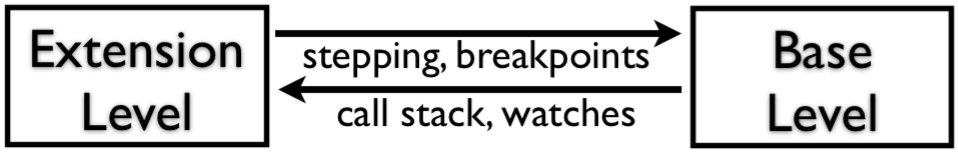
\includegraphics[width=7cm]{./figures/two-levels.png} 
    \vspace{-2mm}
    \caption{Flow of debug information between base and
    extension level~\cite{DBLP:conf/adaEurope/AdaEuropeDeb}}
  \label{infoFlow}
  \vspace{-2mm}
\end{figure}


\subsection{Architecture}

The debugger architecture can be separated into two different aspects: First, a
\ac{DSL} and a set of interfaces for describing the debugging semantics of
language constructs. Second, a runtime for executing those descriptions and this
way performing the mapping described in the~\fig{infoFlow}. 

You can find further information about the architecture and how it is
implemented with \ac{MPS} in \cite{DBLP:conf/adaEurope/AdaEuropeDeb}. In this
section we discuss the specification part, since that is essential for
understanding how debuggers are build and later tested.

\fig{specabs} shows the meta-model used for specifying debugging semantics of
language constructs. Each node is represented in \ac{MPS} by an interface, which
is implemented by the respective language construct.

\noindent \textbf{Breakpoints} \ic{Breakable}s are consturcts on which we can
set breakpoints, \eg statements.

\noindent \textbf{Watchables} \ic{WatchProvider} is something that is either
translated to a lower level watchable (\eg a global variable) or represents a watchable on the
extension-level.
Those \ic{WatchProvider}s live inside \ic{WatchProviderScope} (\eg a
statement list), which can be nested. 

\noindent \textbf{Stepping} Lower level breakpoints are used for realizing
stepping behavior (approach is based on~\cite{Wu06grammar}). The concrete
stepping implementation is encapsulated in \ic{SteppingStrategies}. Those strategies are
contributed by \ic{Steppable}s, which are langauge constructs,
on which we can step over or into (\eg an expression statement). 
Step into is possible on them, if they contain \ic{StepIntoable}s
(\eg a function call). \ic{Steppable} can be contained inside a
\ic{SteppableComposite} (\eg a statement list).

\noindent \textbf{Call Stack} A \ic{StackFrameContributor} is
something that has callable semantics on the extension-level or is
translated to a lower-level callable. While the latter category does not
contribute any \ic{StackFrame}s to the call stack, the other category
contributes one to many \ic{StackFrame}s.

\begin{figure}[h]
  \vspace{-2mm}
  \centering
    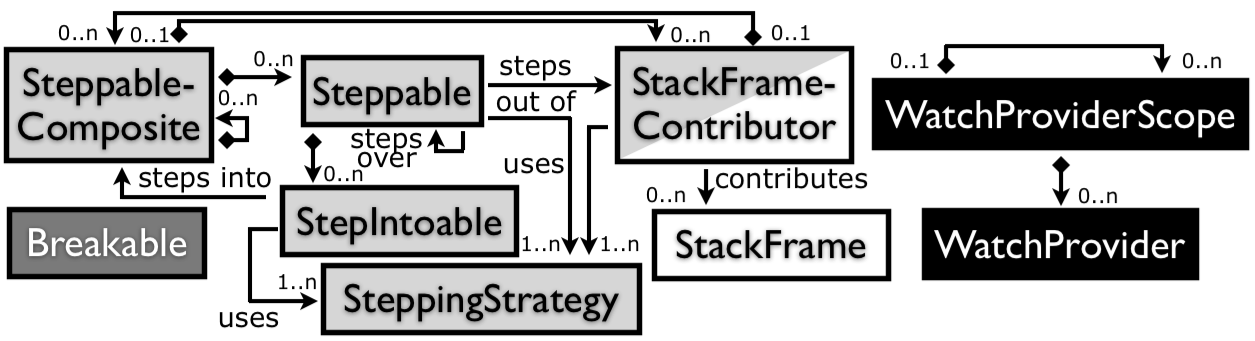
\includegraphics[width=9cm]{./figures/debugger-concepts.png} 
    \vspace{-2mm}
    \caption{Meta-model used for specying the debugging semantics of language
    constructs~\cite{DBLP:conf/adaEurope/AdaEuropeDeb}. Colors indicate the
    different aspects.} 
  \label{specabs}
  \vspace{-2mm}
\end{figure}

The specification \ac{DSL} is a language extension for MPS' Base Language,
which is an implementation of Java. It is used for describing three
debugging aspects: stepping, lifting of call stack and program state. Further
information about the language can be found in
\cite{DBLP:conf/adaEurope/AdaEuropeDeb}. We will later use this \ac{DSL} for
building debugging support for our two language extensions. 


\subsection{Building Debugging Behavior}

We describe in this section the implementation of minimal debugging behavior for
the lanuages described in \sect{languageImplementation}. The mbeddr debugger
comes with a \ac{DSL} for specifying the debugging behavior. 
We will use the abstractions shown in \fig{specabs} and the \ac{DSL} for
building debug support for both languages from \sect{languageImplementation}.

\parhead{Breakpoints}  We want to be able to set breakpoints on instances of
\ic{ForEachStatement} and \ic{AssertStatement}.
For being able to, we need to implement the marker interface \ic{IBreakable} in
both concepts. Since both concepts
are derived from \ic{Statement} and this concept already implements this
interface, we can already set breakpoints on instances of them.
Hence, no further work is necessary.

\parhead{Call Stack} For lifting the call stack we need to specify, which
concepts have callable semantics or are generated to C functions. 
\ic{TestCase} has callable semantics and is trasnalted to a C
function. In contrast, \ic{ExecuteTestExpression} does not have callable
semantics, but is translated to a C function. We therefore implement 
\ic{IStackFrameContributor} in both concepts, but differently.

In the debugger runtime we link instances of \ic{ExecuteTestExpression} to
low level stack frames by implementing \ic{contributeFrameMappings} this way:

\begin{lstlisting}[language=mbeddr]
contribute frame mapping for frames.select(name=getName());
\end{lstlisting}

Further, we return \ic{false} in \ic{isDSLStackFrame}. This query
hides the stack frame from the high-level call stack.

The mapping for \ic{TestCase} is more complex. Here we also start similarly by
linking the low level stack to the \ic{TestCase} instance by
implementing \ic{contributeFrameMappings}. Next, we return \ic{true} in
\ic{isDSLStackFrame}, since the frame should be shown in high level stack.
Finally, \ic{getStackFrameName} returns the name of the actual \ic{TestCase}.
Consider our example \lst{lst:generatedForEach}, where we would lift the frame
\ic{test\_forEach} to \ic{forEach}.

\parhead{Stepping} As described before, stepping is implemented based on setting
low-level breakpoints on the location where execution should suspend after
performing the stepping command. \ic{AsserStatement} is a \ic{Statement}, which
provides already step over behavior, therefore we only need to implement step
into in \ic{contributeStepIntoStrategies}:

\begin{lstlisting}[language=mbeddr]
break on nodes to step-into: this.expr;
\end{lstlisting}

This statement from our debugger \ac{DSL} searches in \ic{this.expr} (the
assert condition in the \ac{AST}) for instances of \ic{StepIntoable} and
collects their step into strategies. 

Next, we implement \ic{StepIntoable} in \ic{TestCaseRef}. In 
\ic{contributeStepIntoStrategies} we put a breakpoint on the first statement
inside the \ic{TestCase}'s body:

\begin{lstlisting}[language=mbeddr]
break on node: this.testcase.body.statements.first;
\end{lstlisting}

In terms of stepping is the implementation of our \ic{ForEachStatement} more
complex. Since this statement contains other statements inside its body,
we implement both, \ic{Steppable} (transitive via \ic{Statement}) and
\ic{SteppableComposite}. We overwrite \ic{contributeStepOverStrategies} and
(1) delegate to our \ic{SteppableComposite} to break on the next statement and
(2) on the body (a \ic{StatementList}):
\begin{lstlisting}[language=mbeddr]
  break on next(drops-frame = false); 
  break on node: this.body; 
\end{lstlisting}

Next, \ic{contributeStepIntoStrategies} is overwritten by searching in \ic{len}
aand \ic{array} (both are \ic{Expression}s) for \ic{StepIntoables}:
\begin{lstlisting}[language=mbeddr]
  break on nodes to step-into: this.len; 
  break on nodes to step-into: this.array; 
\end{lstlisting}

Finally, we implement \ic{contributeStepOverStrategiesForChildren} for our
contained \ic{Steppables}. This method is invoked when stepping inside the
\ic{ForEachStatement}:

\begin{lstlisting}[frame=single,language=mbeddr]
  break on next(drops-frame = dropsFrame); 
  break on node: this.body; 
\end{lstlisting}

\parhead{Watches} For the lifting of watchables, we only care about
\ic{TestCase} and \ic{ForEachStatement}. \ic{ExecuteTestExpression} is also
translated to lower level watchables, but these are not considered since the
corresponding stack frame is not shown in the call stack. \ic{TestCase}
generates the \ic{LocalVariable} \ic{\_fails} we want to hide via the following
\ic{DSL} construct:

\begin{lstlisting}[frame=single,language=mbeddr]
hide local variable with identifier "\_fails";
\end{lstlisting}

Next, \ic{ForEachStatement} hides \ic{LocalVariable} \ic{\_fails} in the same
way as \ic{TestCase}. In addition, we want to show value of \ic{it} by using the
\ic{map by name} construct:

\begin{lstlisting}[frame=single,language=mbeddr]
map by name "\_it" to "it" 
  type mapper: this.array.type:ArrayType.baseType 
  icon provider: this 
  C variable kinds: local variable 
  category name: "local variables" 
  highlighted node: this
\end{lstlisting}

We lift a local variable with name "\_it" to "it" and query the
watchable value from  array's base type. In addition, we provide an icon (shown
in the view), group the watchable inside the view with other local variables
and highlight the \ic{ForEachStatement} when someone click on the
watchable.